% A LaTeX (non-official) template for ISAE projects reports
% Copyright (C) 2014 Damien Roque
% Version: 0.2
% Author: Damien Roque <damien.roque_AT_isae.fr>

\documentclass[a4paper,12pt]{book}
\usepackage[utf8]{inputenc}             % The input file is in utf-8
\usepackage{marvosym}                   % This package provides some symbols. The € is 
\DeclareUnicodeCharacter{20AC}{\EUR{}} 
\usepackage[utf8]{inputenc}
\usepackage[T1]{fontenc}
\usepackage[frenchb]{babel} % If you write in French
%\usepackage[english]{babel} % If you write in English
\usepackage{a4wide}
\usepackage{graphicx}
\graphicspath{{images/}}
\usepackage{subfig}
\usepackage{tikz}
\usepackage{float} 
\usetikzlibrary{shapes,arrows}
\usepackage{pgfplots}
\pgfplotsset{compat=newest}
\pgfplotsset{plot coordinates/math parser=false}
\newlength\figureheight
\newlength\figurewidth
\pgfkeys{/pgf/number format/.cd,
set decimal separator={,\!},
1000 sep={\,},
}
\usepackage{ifthen}
\usepackage{ifpdf}
\ifpdf
\usepackage[pdftex]{hyperref}
\else
\usepackage{hyperref}
\fi
\usepackage{color}
\hypersetup{%
colorlinks=true,
linkcolor=black,
citecolor=black,
urlcolor=black}

\renewcommand{\baselinestretch}{1.05}
\usepackage{fancyhdr}
\pagestyle{fancy}
\fancyfoot{}
\fancyhead[LE,RO]{\bfseries\thepage}
\fancyhead[RE]{\bfseries\nouppercase{\leftmark}}
\fancyhead[LO]{\bfseries\nouppercase{\rightmark}}
\setlength{\headheight}{15pt}

\let\headruleORIG\headrule
\renewcommand{\headrule}{\color{black} \headruleORIG}
\renewcommand{\headrulewidth}{1.0pt}
\usepackage{colortbl}
\arrayrulecolor{black}

\fancypagestyle{plain}{
  \fancyhead{}
  \fancyfoot[C]{\thepage}
  \renewcommand{\headrulewidth}{0pt}
}

\makeatletter
\def\@textbottom{\vskip \z@ \@plus 1pt}
\let\@texttop\relax
\makeatother

\makeatletter
\def\cleardoublepage{\clearpage\if@twoside \ifodd\c@page\else%
  \hbox{}%
  \thispagestyle{empty}%
  \newpage%
  \if@twocolumn\hbox{}\newpage\fi\fi\fi}
\makeatother

\usepackage{amsthm}
\usepackage{amssymb,amsmath,bbm}
\usepackage{array}
\usepackage{bm}
\usepackage{multirow}
\usepackage[footnote]{acronym}

\newcommand*{\SET}[1]  {\ensuremath{\mathbf{#1}}}
\newcommand*{\VEC}[1]  {\ensuremath{\boldsymbol{#1}}}
\newcommand*{\FAM}[1]  {\ensuremath{\boldsymbol{#1}}}
\newcommand*{\MAT}[1]  {\ensuremath{\boldsymbol{#1}}}
\newcommand*{\OP}[1]  {\ensuremath{\mathrm{#1}}}
\newcommand*{\NORM}[1]  {\ensuremath{\left\|#1\right\|}}
\newcommand*{\DPR}[2]  {\ensuremath{\left \langle #1,#2 \right \rangle}}
\newcommand*{\calbf}[1]  {\ensuremath{\boldsymbol{\mathcal{#1}}}}
\newcommand*{\shift}[1]  {\ensuremath{\boldsymbol{#1}}}

\newcommand{\eqdef}{\stackrel{\mathrm{def}}{=}}
\newcommand{\argmax}{\operatornamewithlimits{argmax}}
\newcommand{\argmin}{\operatornamewithlimits{argmin}}
\newcommand{\ud}{\, \mathrm{d}}
\newcommand{\vect}{\text{Vect}}
\newcommand{\sinc}{\ensuremath{\mathrm{sinc}}}
\newcommand{\esp}{\ensuremath{\mathbb{E}}}
\newcommand{\hilbert}{\ensuremath{\mathcal{H}}}
\newcommand{\fourier}{\ensuremath{\mathcal{F}}}
\newcommand{\sgn}{\text{sgn}}
\newcommand{\intTT}{\int_{-T}^{T}}
\newcommand{\intT}{\int_{-\frac{T}{2}}^{\frac{T}{2}}}
\newcommand{\intinf}{\int_{-\infty}^{+\infty}}
\newcommand{\Sh}{\ensuremath{\boldsymbol{S}}}
\newcommand{\C}{\SET{C}}
\newcommand{\R}{\SET{R}}
\newcommand{\Z}{\SET{Z}}
\newcommand{\N}{\SET{N}}
\newcommand{\K}{\SET{K}}
\newcommand{\reel}{\mathcal{R}}
\newcommand{\imag}{\mathcal{I}}
\newcommand{\cmnr}{c_{m,n}^\reel}
\newcommand{\cmni}{c_{m,n}^\imag}
\newcommand{\cnr}{c_{n}^\reel}
\newcommand{\cni}{c_{n}^\imag}
\newcommand{\tproto}{g}
\newcommand{\rproto}{\check{g}}
\newcommand{\LR}{\mathcal{L}_2(\SET{R})}
\newcommand{\LZ}{\ell_2(\SET{Z})}
\newcommand{\LZI}[1]{\ell_2(\SET{#1})}
\newcommand{\LZZ}{\ell_2(\SET{Z}^2)}
\newcommand{\diag}{\operatorname{diag}}
\newcommand{\noise}{z}
\newcommand{\Noise}{Z}
\newcommand{\filtnoise}{\zeta}
\newcommand{\tp}{g}
\newcommand{\rp}{\check{g}}
\newcommand{\TP}{G}
\newcommand{\RP}{\check{G}}
\newcommand{\dmin}{d_{\mathrm{min}}}
\newcommand{\Dmin}{D_{\mathrm{min}}}
\newcommand{\Image}{\ensuremath{\text{Im}}}
\newcommand{\Span}{\ensuremath{\text{Span}}}

\newtheoremstyle{break}
  {11pt}{11pt}%
  {\itshape}{}%
  {\bfseries}{}%
  {\newline}{}%
\theoremstyle{break}

%\theoremstyle{definition}
\newtheorem{definition}{Définition}[chapter]

%\theoremstyle{definition}
\newtheorem{theoreme}{Théorème}[chapter]

%\theoremstyle{remark}
\newtheorem{remarque}{Remarque}[chapter]

%\theoremstyle{plain}
\newtheorem{propriete}{Propriété}[chapter]
\newtheorem{exemple}{Exemple}[chapter]

\parskip=5pt
%\sloppy

\begin{document}
\let\cleardoublepage\clearpage
%%%%%%%%%%%%%%%%%%
%%% First page %%%
%%%%%%%%%%%%%%%%%%


\begin{titlepage}
\begin{center}
\vfill

{\large Université de Paris Ouest Nanterre La Défense}\\[0.5cm]

{\large Mémoire}\\[0.5cm]



% Title
\rule{\linewidth}{0.5mm} \\[0.4cm]
{ \huge \bfseries Prédiction de la stratégie de récupération d'un service Web composite\\[0.4cm] }
\rule{\linewidth}{0.5mm} \\[1.5cm]

\vfill
\vfill
\vfill

% Author and supervisor
\noindent
\begin{minipage}{0.7\textwidth}
  \large
    \emph{Réalisé par :}\\
- Nadia \textsc{MASLOUHI}\\
\end{minipage}%
\begin{minipage}{0.5\textwidth}
   \large
    \emph{Encadrants :} \\
- Mme.~Castillo Marta \textsc{RUKOZ}
\end{minipage}

\vfill
\vfill
\vfill
\vfill
\vfill
\vfill
% Bottom of the page

\end{center}
\end{titlepage}
\clearpage

\chapter*{Remerciements}


Je tiens à remercier toutes les personnes qui m’ont aidée lors de la rédaction de ce mémoire. 

...

\tableofcontents
\listoffigures
%%%%%%%%%%%%%%%%%%%%%%%%%%%%%%%%%%%%%%%%%%%%
%%% Content of the report and references %%%
%%%%%%%%%%%%%%%%%%%%%%%%%%%%%%%%%%%%%%%%%%%%

\mainmatter
\pagestyle{fancy}


\vspace{1cm}


\chapter{introduction}

Les web services sont un ensemble de fonctionnalités de programmes informatiques permettant à des applications et des systèmes de fonctionner et d'échanger des informations à distance.

Un utilisateur de web service peut être satisfait par la réponse d’un web service comme il ne le peut pas être, si sa requête est beaucoup plus complexe, et dans ce cas la solution c’est d’utiliser des web services composite, obtenu en combinant un ensemble des web services disponibles.

Pendant l'exécution des Web services composites (CWS), l’un des Web services composant peut échouer ou tomber en panne, c’est pour cela il existe des différentes stratégies de récupération pour dépasser le problème (RollBack, Substitution, Cheekpoint).

Chaque stratégie se comporte d’une manière différente selon les différents scénarios d’exécution, ce qui influence sur la qualité de service.

Notre objectif est de déterminer d’une manière dynamique  la meilleure stratégie de récupération  dans le cas d’une défaillance d’un Web service, en analysant  plusieurs niveaux d'informations comme l’état de l'environnement, l’état d'exécution et les différents critères de qualité de service.

Notre étude va se basé sur les outils de Machine Learning pour prédire la meilleure stratégie en cas de défaillance, pour cela il est indispensable de collecter et traiter l’ensemble des données et des informations descriptives de l’environnement, l’exécution, et les critères de qualité de service, pour cet étape on va travailler avec l’outil Pentaho.


\chapter{Concepts}

\section{Introduction}

Un web Service Composite est  le résultat des différentes combinaisons de plusieurs web Services qui vise à répondre aux requêtes complexes des utilisateurs.
Pendant l'exécution des Web services composites (CWS), un Web service composant (WS) peut échouer ou tomber en panne, et pour cela il existe des stratégies qui permettent la réparation du problème telles que  la réexécution du WS,la réplication,Récupération arrière ou point de contrôle.
La question qui se pose, quelle est la meilleure stratégie de récupération ? 
( a revoir ) 

\section{Service Web Composite}

L'architecture orientée services ( SOA Services Oriented Architecture) est une architecture logicielle qui met en oeuvre un ensemble de services simples (Composants logiciels).

L'architecture orientée services a pour objectif la décomposition d'une fonctionnalité en un ensemble de fonctions basiques, appelées services, fournies par des composants et la description des interactions entre ces services.


\begin{figure}[H]
\begin{center}
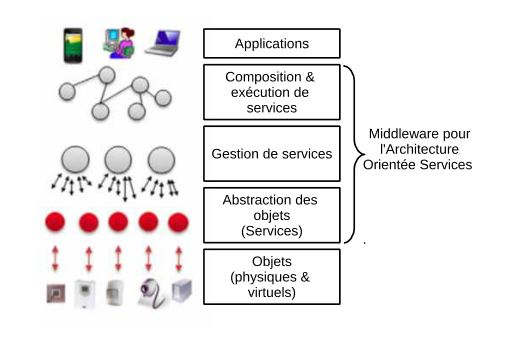
\includegraphics[width=1\linewidth]{images/MiddlewareSOA.jpg}
\end{center}
\caption{Middleware pour l’Architecture Orientée Services}
\label{fig:1}
\end{figure}

La figure 1 illustre l'architecture orientée services, la contribution de ce mémoire se positionne dans la couche Composition et exécution de services.
Cette couche fournit une composition des services et se charge du suivi de l’exécution de ces services composites. Un aspect important de cette couche est la résilience aux
pannes et l’adaptation en fonction des changements dans le système \cite{1}.



D'après l'architecture vu précédemment, Un service Web composite peut être définis comme un  résultat d’une composition de plusieurs Web services, et qui peut à son tour entrer dans une autre composition.
Les  services web composites ont pour objectif  la production des services complexes pour répondre à des demandes d’utilisateurs complexes. 

La structure d’un Web service composite peut être générée manuellement ou automatiquement. Selon les requêtes demandées, les utilisateurs peuvent spécifier manuellement comment les fonctionnalités des Web service seront combinées ou bien  un composeur qui prend la responsabilité d’une génération automatique des Web service Composite en fonction de la demande, pour qu’ils seront finalement exécuté par un moteur d’exécution.


\begin{figure}[H]
\begin{center}
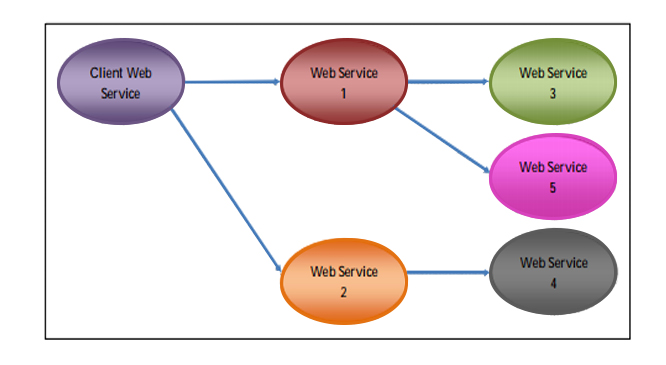
\includegraphics[width=1\linewidth]{images/CWS.jpg}
\end{center}
\caption{Web service composite}
\label{fig:2}
\end{figure}



Les Web services composite peuvent être représentés sous différents formes et structures en indiquant l’ensemble des informations et instructions relatives, comme l’ordre d’exécution et le comportement des Web services composants ainsi que les flux de données  et de contrôle.
La représentation peut être sous forme de Workflows, Graph ou réseau de Petri.



Les différents travaux et articles scientifiques sur la composition des services Web considèrent la composition de services Web comme étant un moyen efficace 
pour créer, exécuter, et maintenir des services qui dépendent d’autres services. Les auteurs ont défini le cycle de vie d’une composition de services Web reposant à partir de six activités [Benatalla] \cite{6}: 

- L’encapsulation de services natifs (Wrapping services): Cette première activité permet de  s’assurer que tout service peut être appelé lors d’ une composition, indépendamment de son  modèle de données, de son format de message, et de son protocole d’interaction. 


- L’établissement d’accord d’externalisation (Setting outsourcing agreements): Cette seconde activité consiste à négocier, établir, et appliquer des obligations contractuelles entre les services.


- L’assemblage de services composants (Assembling composite services):Cette activité permet  de spécifier, à un haut niveau d’abstraction, l’ensemble des services à composer afin d’atteindre  l’objectif attendu. Cet assemblage comporte une phase d’identification des services et de spécification de leurs interactions conformément aux descriptions et aux accords entre services. 


- L’exécution de services composants (Executing services):Cette activité consiste en l’exécution des spécifications de la composition précédemment définies. 


- Le contrôle de l’exécution de services composites (Monitoring services): La phase de contrôle permet de superviser l’exécution de la composition en vérifiant, par exemple, l’accès aux services, les changements de statut, les échanges de messages. Ce contrôle permet de détecter des violations de contrats, de mesurer les performances des services appelés et de prédire des exceptions. 


- L’évolutivité des services (Evolving services):Cette dernière phase permet de faire évoluer la composition en modifiant les altérations de l’organisation de services, en utilisant de nouveaux  services, ou en prenant en compte les retours de la phase de contrôle. \cite{6}



Dans ce mémoire, nous considérons les services avec leurs définition général c'est à dire des opérations exposées
sur Internet qui sont indépendantes de leur mise en œuvre. les détails d’implémentations telles que SOAP ou REST sont hors du domaine d’investigation de ce mémoire.

Les services sont décrits en fonction de leur fonctionnalités et des critères de qualité de service (QoS). Dans notre cas, la fonctionnalité d’un service est donnée par les paramètres d’entrée et de sortie.

\subsection { Qualité de Service }

La qualité de service (QoS Quality of Service) décrivent les caractéristiques non fonctionnelles du service Web, autrement dits la mesures dans laquelle un ensemble de caractéristiques répond à un besoin ou une attente.

nous considérons les trois critères de qualité suivantes \cite{2} :

- Temps de réponse: le temps estimé nécessaire pour achever une invocation de service ; qui est, la durée entre une demande de service et la réponse du service correspondant.

- Disponibilité : la probabilité d’obtenir une réponse correcte après une invocation de service. Cela inclut la probabilité que le service est disponible, qu’il s’exécute correctement, et que la transmission de message entre le
service et le demandeur a réussi.
 
- Prix: une mesure du coût d’exécution d’un service.


\section{Exécution tolérante aux pannes}

La tolérance aux pannes est la manière dont un système informatique, un système électronique ou un réseau répond à une défaillance matérielle ou logicielle. Le terme fait essentiellement référence à la capacité d'un système à prendre en compte les défaillances ou les dysfonctionnements d’un ou de plusieurs de ses composants, tout en fournissant un service ininterrompu, et cette capacité peut être fournie par un logiciel, un matériel ou une combinaison des deux.

Le but est d'éviter une panne catastrophique qui pourrait résulter d'un seul point de défaillance. 

\subsection{Défaillance des Web Service Composite}

Comme toutes les technologie, Les Web services Composite ne peuvent pas s’échapper aux défaillances d’exécution à 100 \%, car des pannes peuvent survenir à tout moment au niveau du matériel, du moteur d’exécution ou tout simplement du défaillance d’un Web service composant.
Cependant les Web Services Composite fonctionne potentiellement de manière réduite (en mode dégradé).


Soulever et relever les défis posés par les problématiques de résilience et de fiabilité des web services composite nécessite en premier lieu l’analyse  des caractéristiques des pannes dans  leur exécution.
On peut distinguer principalement dans l’environnement d’exécution des Web services Composites deux classe de pannes \cite{2}. 

    - Panne de nature silencieuse: (silent faults) Sont les pannes indétectables, ou qui sont détectées après une très grande durée depuis leurs déclenchements ce qui implique nécessairement que le résultat fourni est incorrect. 
    Ces pannes sont génériques pour tous les WS. Ils empêchent les WS de répondre.


    - Panne de nature logique: (Logic fault): Contrairement au pannes silencieuse, les panne logiques sont spécifiques aux différents Web service, et les attributs des entrées représente la cause principale de ces pannes.
    Ce genre d’erreur est difficile d’être identifié par le moteur d’exécution des Web services composites.

\subsection{Exécution tolérante aux pannes des CWS}

Le contrôle d'exécution des Web services composites peut être centralisé c’est à dire un coordinateur qui va jouer le rôle de la gestion de toute l’exécution,  ou distribué dans lequel le processus d’exécution de déroule avec la collaboration de plusieurs participants sans un coordinateur central. Comme il peut être attaché aux web services composants ou indépendant.
Certaines méthodes indépendantes de tolérance aux pannes dont apparus, telles que les propriétés transactionnelles et la réplication. Les propriétés transactionnelles décrivent implicitement le comportement des services web en cas d'échec, et sont utilisées pour garantir la propriété transactionnelle d’atomicité.

Les propriétés transactionnelles les plus utilisées pour les services web sont pivot, compensable, et retriable [Rafael Enrique Angarita Arocha],[modeling dinamic ...] \cite{1}. 
 
 - Pivot(p) : un service est appelé pivot si ses effets restent pour toujours
et ne peuvent pas être annulés sémantiquement une fois qu’il a terminé son exécution avec succés. Il s’agit de la propriété transactionnelle la plus basique.

- Compensable (c) : un service est compensable s’il existe un autre service qui peut sémantiquement annuler son exécution s'il n'as pas pu terminer avec succès.  
 
- Retriable (r) : un service est retriable s’il garantit une exécution réussie après un nombre fini d’invocations. Cette propriété doit être combinée avec les propriétés pivot ou compensable, créant les propriétés pivot-retriable (pr) et compensable-retriable (cr).

Les services Web composites sont construit à partir d'un ensemble des service qui offrent des propriétés transactionnelles garantissent la cohérence su système et ont une propriété transactionnelle agrégée comme suit [Rafael Enrique Angarita Arocha]: 

- Atomique : un service composite est atomique si au moins un de ses services composant est pivot ou pivot retriable. Lorsqu’un service composite atomique se termine avec succès, ses effets demeurent pour toujours et ils ne peuvent pas être annulées. Si l’un de ses services composants tombe en panne, le système est laissé dans un état sémantiquement similaire à celui qu’il avait avant l’exécution du service composite.


- Compensable : un service composite est compensable si tous ses services composants sont compensables. Cela signifie qu’il existe un autre service composite, contenant les services qui compensent les services du service composite compensable, qui peut annuler sémantiquement les effets du service composite compensable après son exécution réussie. Comme pour le service composite atomique, si l’un de ses service composants tombe en panne, le système est laissé dans un état sémantiquement similaire à celui qu’il avait avant l’exécution du service composite compensable.


- Retriable : un service composite est retriable si tous ses services composants sont retriables. Un service composite retriable garantit l’exécution réussie après un laps de temps limité. Cette propriété doit être combinée avec les propriétés atomiques ou compensables, pour créer les propriétés atomique-retriable (ar) et compensable-retriable (cr).


\section{Mécanisme de récupération}

En présence des pannes, les propriétés transactionnelles fournis par les services ont une importance dans la création des services composites fiables, car ils assurent un état cohérent de l'ensemble du système.

La stratégie de reprise d'une exécution de service composite dépend de la propriété transactionnelle des services composants.
Les principaux mécanisme de récupération sont \cite{1} : 

- Récupération en arrière : c'est l'opération de restauration de l’état du système avant l’exécution du service composite ; c’est-à-dire, tous les effets produits par le service en panne sont annulées par rollback, et les effets des services exécutés avant la panne sont sémantiquement annulés en utilisant des techniques de compensation (Fig (a)).


- Récupération en avant : c'est l'opération qui permet la réparation du panne afin que le  service composite peut poursuivre son exécution ; les techniques utilisées pour fournir une récupération en avant sont le réessayage de l’invocation de service ou le remplacement du service (Fig (b)).


- Récupération sémantique : elle a le même mécanisme que la récupération en arrière, sauf que la récupération sémantique est effectuée après une exécution réussie d’un service composite en compensant l’exécution de ses services composants. L’idée est de laisser le système dans un état sémantiquement proche de l’état qu’il avait avant l’exécution du service composite (Fig (c))

- Checkpointing : c'est l'opération qui permet si une panne survient de continuer l’exécution de la partie du service composite qui n’a pas été affecté par cette panne, tout en retardant l’exécution de la partie affectée (Fig (d))

\begin{figure}[H]
\begin{center}
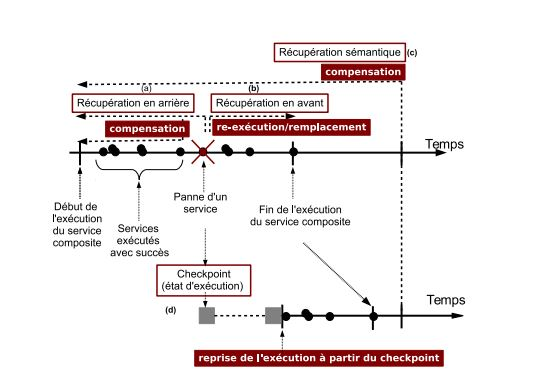
\includegraphics[width=1\linewidth]{images/techsreparation.jpg}
\end{center}
\caption{Stratégies de récupération \cite{1}}
\label{fig:3}
\end{figure}

\vspace{1cm}

\chapter{État de l'art}

\section{Introduction}

Ce chapitre présente l'étude existante avec son ensemble d'approches pour une exécution fiable des services Web composites.
Cet étude consiste l'exécution auto-corrective (self-healing) d'une manière dynamique et automatique, elle vise le même objectif de ce mémoire mais les méthodologies changent. 

Dans cette étude les chercheurs ont proposé l'approche de l'auto-corrective  (self-healing) qui se base sur les propriétés transactionnelles comme un concept de base pour une tolérance aux pannes automatique, et se base aussi sur les agents à base de connaissances.

Dans un premier temps les auteurs ont proposé une approche pour l'exécution tolérante aux pannes des services Web composite basée sur la récupération en avant et en arrière, et définie par le formalisme de réseaux de Petri Colorés, ensuite sur le même formalisme la deuxième approche consiste la proposition d'un mécanisme de point de contrôle, et finalement après une étude sur l'impact des différentes stratégies de récupération sur les services Web composite, la troisième approche apporte un modèle de décision dynamique de la stratégie de récupération en terme d'impact sur la qualité de service pour la tolérance aux pannes de services Web composites.


\section{Contrôle d'exécution de services Web composites}

En utilisant les réseaux de Petri Colorés les auteurs ont formalisé les services Web composites, leur exécution, et leurs stratégies de tolérance aux pannes, et il ont proposé un framework pour une exécution distribuée fiable et tolérante aux pannes pour les services Web Composites.

Le framework est composé de deux types de composants \cite{1} \cite{5}: 

- Un Coordinateur d'Agents : Composant responsable de la gestion des aspects globaux d'exécution des services Web composites.

- Agents de Service : ils exécutent les services et sont en charge du contrôle de l'exécution et de la tolérance au pannes.

Cette approche fournis les mécanismes de récupération en arrière par compensation, en avant par re-exécution de service et remplacement, la réplication, et le checkpointing, et assure une exécution tolérante aux pannes basé sur un modèle d'exécution distribué.

L'exécution des services Web composite peut être \cite{3} : 

- Séquentiel : Les services se basent sur les résultat des services précédents, et ne peuvent être invoqués tant que les services précédent ne sont pas terminés.

- Parallèle : Les services peuvent être invoqués d'une manière simultanée, car il n'y a pas des dépendances de flux de données entre eux.

Ces deux scénarios d'exécution ont un effet sur la propriété transactionnelle globale du service Web composite, pour cela il faut suivre le flux d'exécution défini par le graphe du service composite pour s'assurer que l'exécution séquentielle et parallèle satisfont la propriété transactionnelle globale.

\subsection{Architecture du Framework}

Les chercheurs ont proposé un Framework dont l'exécution du service composite est gérée par un Coordinateur d'Agents et une collection d'Agents de services, organisés dans architecture trois tiers.

\begin{figure}[H]
\begin{center}
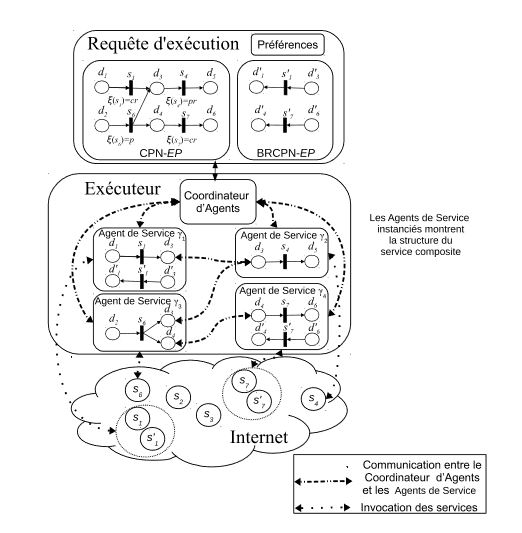
\includegraphics[width=1\linewidth]{images/architectureFrmwork.jpg}
\end{center}
\caption{Architecture d'exécution \cite{1}}
\label{fig:4}
\end{figure}


L’architecture du Framework est composée de trois niveaux principaux:

Le premier niveau : Le coordinateur d’agents reçoit le service composite et son graphe de compensation correspondant, qui sont représentés sous forme des réseau de Pétri Colorés, qui peuvent être générés d'une manière automatique ou manuelle.
Dans ce niveau le Coordinateur reçoit aussi une propriété qui lui indique si le mécanisme de checkpointing est activé ou non.

Le deuxième niveau: Le coordinateur d'Agents lance un Agent de Service pour chaque service composant du service Web composite, chaque agent de service sera responsable du contrôle de l'exécution de son service, ses rôles sont les suivants \cite{1}:

    - Responsabilité de l'invocation de services ;

    - Surveillance de l'exécution des services correspondants ;
    
    - Envoi des résultat selon le flux d'exécution ;
    
    - Lancement des stratégies de tolérance aux pannes en cas de panne.

Le troisième niveau : consiste l'interaction des agents de services avec l'ensemble des services correspondants.

L'objectif de cet architecture est de répartir la responsabilité de l'exécution d'un service Web composite à travers de plusieurs agents de service, pour que le modèle logique de l'exécuteur proposé permet une exécution distribuée et une indépendance de la mise en oeuvre 

\section{Modélisation des stratégies de récupération basées sur QoS}

Après les évolutions des recherches, les auteurs ont découvert a travers leur étude qu'il y a des impacts des différentes stratégies de récupération sur les services Web composite et plus précisément sur sa qualité de service (QoS). C'est pour cela ils ont décidé de proposer une approche pour une décision dynamique des stratégies de récupération.

Pour fournir un choix dynamique de la stratégie de tolérance aux pannes, les auteurs ont proposé une approche auto-corrective (Self-Healing) pour les services Web composites.
Dans l'auto-correctif les agents de services sont des agents basés sur des connaissances, c'est à dire ils sont basés sur l'ensemble des information qu'ils ont sur le service Web composite, sur eux mêmes, et sur ce qui est attendu et ce qu'il se passe réellement pendant l'exécution, pour qu'ils puissent finalement faire la sélection de la stratégie de tolérance aux pannes.

Indépendamment de la technique utilisée pour l'estimation des critères de Qualité de service,ils ont proposé que chaque service Web est annoté avec son temps d'exécution estimé, son prix, sa réputation et sa propriété transactionnelle. Grâce aux critères des services composants, il est possible de calculer la Qualité de service d'un service Web composite en calculant des différents critères.

Sur cette base, la conception sera sous forme d'une boucle d'auto-guérison/auto-correction par agent de service pour effectuer la détection, le diagnostic et la récupération d'une manière décentralisée \cite{1}.


\begin{figure}[H]
\begin{center}
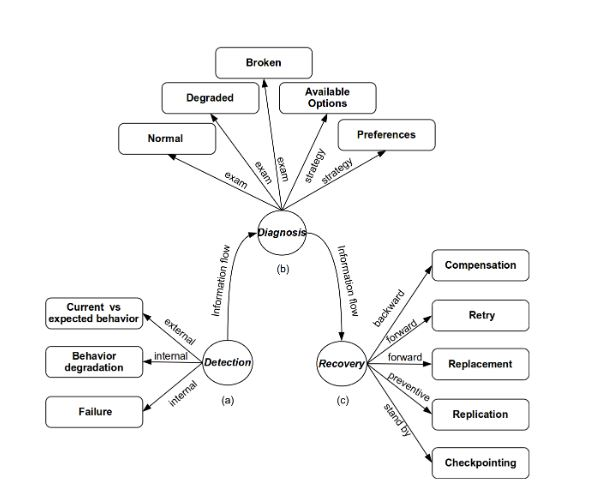
\includegraphics[width=1\linewidth]{images/Boucleauto-correctivedesAgentsdeService.jpg}
\end{center}
\caption{Architecture d'exécution \cite{1}}
\label{fig:5}
\end{figure}

- Le composant detection : Dans ce composant, trois sources sont prises en compte une externe et deux internes. 
La source externe consiste l'information sur la Qualité de service attendu, par exemple, le cas où l'utilisateur peut permettre une certaine dégradation de la Qos.
La source interne concerne la dégradation de la Qualité de service des services composants (par exemple, les variations négatives dans le temps d'exécution et le prix), et concerne aussi les pannes de services.

- Le composant diagnosis : ce composant a le rôle d'analyse du problème et la détermination de l'état du service.
Il existe trois diagnostics possibles qui correspondent au trois états d'un système auto-correctif : normal ; degraded ; et broken. Le choix de la stratégie de récupération est influencé par les options disponibles ( par exemple, les propriétés transactionnelles, les services de remplacement disponible, etc.), et influencé aussi par les préférences de l'utilisateur (la QoS attendu, le checkpointing, etc).

- Le composant recovery :  Ce composant prend en charge l'exécution des mécanismes de tolérance aux pannes sélectionnés : la récupération vers l'arrière avec la compensation ; la récupération en avant par la reexécution ou remplacement ; la prévention grâce à la réplication ; ou le retardement d'exécution par le checkpointing.



\section{Évaluation expérimentale }

Les chercheurs ont mis leur approche en évaluation expérimentale, et ça par la mise en oeuvre du Framework  en utilisant un cas d'étude qui consiste un scénario et un environnement.
L'observation du cas d'étude a été sur trois systèmes différent :

Système sans tolérance au pannes : c'est un système qui n'a aucun mécanisme de tolérance aux pannes. et dans le cas ou un des services composants tombe en panne, une exception sera générée et l'exécution sera terminé.

Système transactionnel : c'est un système qui se base sur les propriétés transactionnelles des services composants pour prendre les décisions de récupération.

Système auto-correctif :  c'est un système qui se base sur l'ensemble d'information et règle contenu dans les bases de connaissances des agents de services.


Les résultat de l'évaluation expérimentale ont montré : l'importance et la nécessité d'avoir des mécanisme de tolérance aux pannes pour les services Web composite, ainsi que la manière avec laquelle les deux approches des propriétés transactionnelles et l'auto-corrective gèrent les pannes et prennent la décision de récupération.
L'évaluation expérimentale faite pendant cette étude suggère que la combinaison des propriétés transactionnelles avec des capacités d'auto-corrective permet de donner une intelligence aux systèmes d'exécution pour gérer les exigences de haut niveau pour les exécutions de services Web composites avec une intervention humaine minimale\cite{1}.

\section{Conclusion}

Pendant cette étude, les auteurs ont proposé une approche auto corrective pour l'exécution de services Web composite qui se base sur les propriété transactionnelles des services Web composants ainsi que sur une base d'informations sur les Services Web qui se présente principalement dans la Qualité de chaque service QoS.

L'avantage principale de cette étude c'est la mise en oeuvre des mécanismes de d'exécution et de récupération qui sont capables de fonctionner d'une manière automatique, ces mécanismes sont mis en place a travers un Framework qui se base sur des agents de services qui sont en charge du contrôle de l'exécution  et de la tolérance en pannes, ces agents prennent un ensemble d'informations en entrée pour qu'il puissent les analyser et en déduire des nouvelles informations qui vont permettre une prise de décision lors de l'exécution.

Cet étude est considérée comme une base pour le sujet de recherche du présent mémoire, qui visent le même objectif de l'auto-corrective, et qui se situe dans les principaux perspectives de cette étude.

Le mémoire est l'un des principaux perspectives de l'étude présentée dans l'état de l'art car il se base sur l'ensemble des données générées par le système d'exécution de services Web composites mis en place pendant l'étude expérimentale précédente. Donc l'objectif sera collecter et stocker les données générées, les traiter et les analyser à l'aide des outils de l'auto apprentissage (Machine Learning) pour en pouvoir prédire la bonne décision de stratégie de récupération.





\chapter{La prédiction du mécanisme de récupération}

\section{Introduction}
Notre étude a pour objectif la prédiction de la meilleure stratégie de récupération en cas de pannes dans un Web Service Composite en se basant sur un ensemble d'informations concernant les Web services composé et la qualité de service.

L'approche proposé dans ce présent mémoire se base sur la notion de l'auto-apprentissage (Machine Learning), L'ensemble des données généré dans l'étude précédente cité dans le chapitre "État de l'art", vont être traité et exploité comme des données d'apprentissage, pour qu'on puisse après prédire d'une manière automatique et dynamique le mécanisme de récupération le mieux adapté.

Le présent chapitre décris d'une part les différent problématiques de l'auto-apprentissage ainsi que le type de problématique dans lequel se situe notre approche de prédiction, d'autre part on va présenter les deux étapes principaux de l'approche, le traitement et l'intégration des données en utilisant Pentaho et la prédiction des mécanismes de récupération en appliquant les algorithmes de Machine Learning via l'outil Weka. 


\section{L'auto Apprentissage -Machine Learning- }

L'apprentissage automatique -Machine Learning- est un domaine de l'intelligence artificielle qui consiste en général une manière de traitement d'un ensemble de données pour un apprentissage automatisé de la machine ou de l'ordinateur afin de pouvoir effectuer des opérations complexes.

Un algorithme de machine Learning se différencie des autres algorithmes classiques à travers la notion de l'apprentissage, car un algorithme de Machine Learning s'améliore par lui même à partir des données sans supervision d'un être humain.

Pour bien définir un problème de machine learning, il faut bien définir quatre element principaux: 

- Les données

- La tache à accomplir 

- L'algorithme d'apprentissage

- La mesure de performance


Les données : représente l'ensemble de base d'information sur lesquelles se base l'apprentissage automatique, notre approche se base sur les données générées par le système d'exécution des services Web Composite cité dans l'Etat de l'art.

La tache spécifique : Le Machine Learning a besoin de la définition d'une tâche spécifique à accomplir c'est à dire  qu'est ce qui peut répondre au problème, une tâche peut être sous forme d'une prédiction, identification, recommandation... 

L'algorithme : Après la définition de la tâche spécifique et les données nécessaires pour la traiter, On peut passer à la troisième étape qui consiste le choix d'un algorithme spécifique qui va pouvoir répondre à la tache à partir des données collectée. il existe plusieurs algorithmes de Machine Learning ( Réseau de neurones, Support vector machine, Régression linéaire ... ), le choix de l'algorithme dépend de la nature et le type de la problématique de machine Learning.

La mesure de performance : Une fois l'algorithme est déterminé, il faut choisir une mesure de performance relativement à la tache définie précédemment en s'appuyant sur des métriques précises.  

Un process de Machine Learning passe par deux phases principales, La première phase c'est la phase où l'être humain sera responsable du choix et de l'entraînement de l'algorithme d'apprentissage, pour que le traitement de la tache spécifique sera appris à partir de l'apprentissage (Training set), pour que l'algorithme dans la deuxième phase effectue la tâche lui même.

\begin{figure}[H]
\begin{center}
\includegraphics[width=1\linewidth]{images/auto apprentissage.png}
\end{center}
\caption{Processus du Machine Learning}
\label{fig:6}
\end{figure}

\subsection{Choix de l'algorithme de Machine Learning}

Le choix de l'algorithme auquel  on va avoir besoin de faire appel pour le traitement de la problématique nécessite tout d'abord  la distinction des différents types de problèmes de Machine Learning et les familles d'algorithmes associés avec leurs spécificités.

La première distinction à faire dans les problèmes de Machine Learning, c'est la détermination des problèmes supervisés (supervised learning) et des problèmes non supervisés (unsupervised learning), la seconde consiste la distinction entre un problème de Régression et un problème de Classification.

\subsubsection{Apprentissage supervisé vs non-supervisé}


- L'apprentissage supervisé : exploite exclusivement l'ensemble des données dites annotées de leur sorties pour pouvoir construire un modèle, c'est à dire que chaque donnée est associée à une classe cible ou une catégorie et l'objectif c'est que l'algorithme soit capable de prédire cette classe sur des nouvelles données qui ne sont pas annotées a partir du modèle qui a construit précédemment.

Représentation Mathématique : 
    
    On reçoit en entré des données d'exemple annotées:
    (x1,y1),(x2,y2),(x3,y3), ... et on veut prédire la sortie sur des nouvelles données :  x* --> y* 
    

- L'apprentissage non-supervisé : est beaucoup plus complexe puisque les données d'entrées ne sont pas annotées. l'algorithme d'entraînement va devoir dans ce cas  trouver  les similarités et distinctions au sein de ces données, et à organiser et regrouper ensemble celles qui partagent des caractéristiques communes.

Représentation Mathématique : 
    
    On reçoit en entré uniquement des données brutes de variables aléatoire : x1,x2,x3,... et on veut avoir la relation avec des variables latentes structurelles :  xi --> yi 
    
En plus de ces deux principaux familles d'algorithme (Supervisé/non-Supervisé) il existe d'autre types d'apprentissage, l'apprentissage semi-supervisé qui prend en entré un mélange de données annotées et non annotées et l'apprentissage par renforcement son but est d'apprendre a partir des expériences, en gros l'algorithme de base sur un cycle d'expériences et de récompenses et il s'auto améliore à chaque itération.

\subsubsection{Classification vs Régression }

\begin{figure}[H]
\begin{center}
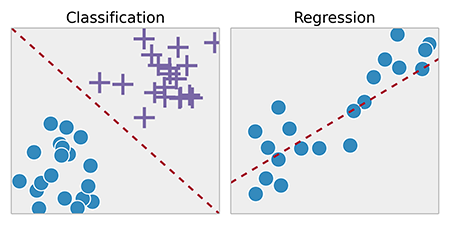
\includegraphics[width=1\linewidth]{images/ClassReg.png}
\end{center}
\caption{Différence entre Classification et Régression}
\label{fig:6}
\end{figure}

- Classification : Chaque observation ou donnée  est associée à une et une seule modalité (appelée classe/catégorie), La classification c'est le type de problème dans lequel la sortie attendu de l'algorithme est discrète c'est à dire elle est sous forme d'une catégorie ou classe.
    
- Régression : La variable de sortie de l'algorithme est quantitatif, c'est à dire elle  prend des valeurs dans un sous-domaine de l’ensemble des nombres réels. exemple: La prédiction de la rentabilité d'une compagne marketing. 


Notre problématique concerne la prédiction de la stratégie de récupération d'un service Web composite, c'est à dire prédire quelle catégorie ou classe de récupération va être mise en oeuvre, ainsi que nos données d'apprentissage sont des données qui sont générées par  un exécuteur des services Web composites vu dans l'étude précédente (Chapitre :État de l'art) et  qui permet de prendre la décision de choix de Mécanisme de récupération ce qui nous permet d'avoir un ensemble des données annotées. 
D'après cet analyse on peut situer notre problème de machine Learning dans la famille des problèmes Supervisés de Classification.

\subsubsection{Les algorithmes de Classification et Supervision}



\section{Construction du modèle de prédiction }

\subsection{Weka}
\subsection{Scikit Learn Python }

\subsection{Mesure de performance}







\appendix


\bibliographystyle{authoryear-fr}
\bibliography{reference}


\end{document}